% !TEX TS-program = XeLaTeX
% use the following command:
% all document files must be coded in UTF-8
\documentclass[english]{textolivre}
% build HTML with: make4ht -e build.lua -c textolivre.cfg -x -u article "fn-in,svg,pic-align"

\journalname{Texto Livre}
\thevolume{18}
%\thenumber{1} % old template
\theyear{2025}
\receiveddate{\DTMdisplaydate{2025}{3}{25}{-1}} % YYYY MM DD
\accepteddate{\DTMdisplaydate{2025}{5}{31}{-1}}
\publisheddate{\DTMdisplaydate{2025}{9}{5}{-1}}
\corrauthor{Lakshmana Rao Pinninti}
\articledoi{10.1590/1983-3652.2025.58320}
%\articleid{NNNN} % if the article ID is not the last 5 numbers of its DOI, provide it using \articleid{} commmand 
% list of available sesscions in the journal: articles, dossier, reports, essays, reviews, interviews, editorial
\articlesessionname{articles}
\runningauthor{Pinninti} 
%\editorname{Leonardo Araújo} % old template
\sectioneditorname{Daniervelin Pereira}
\layouteditorname{Saula Cecília}

\title{Undergraduate ESL students' use and perceptions of ChatGPT for academic writing purposes}
\othertitle{O uso e as percepções de estudantes de graduação em ESL sobre o ChatGPT para fins de escrita acadêmica}
% if there is a third language title, add here:
%\othertitle{Artikelvorlage zur Einreichung beim Texto Livre Journal}

\author[1]{Lakshmana Rao Pinninti~\orcid{0000-0003-0300-6339}\thanks{Email: \href{mailto:lakshman_ma007@yahoo.co.in}{lakshman\_ma007@yahoo.co.in}}}
\affil[1]{Indian Institute of Technology Kanpur, Department of Humanities and Social Sciences, Kanpur, India.}

\addbibresource{article.bib}
% use biber instead of bibtex
% $ biber article

% used to create dummy text for the template file
\definecolor{dark-gray}{gray}{0.35} % color used to display dummy texts
\usepackage{lipsum}
\SetLipsumParListSurrounders{\colorlet{oldcolor}{.}\color{dark-gray}}{\color{oldcolor}}

% used here only to provide the XeLaTeX and BibTeX logos
\usepackage{hologo}

% if you use multirows in a table, include the multirow package
\usepackage{multirow}

% provides sidewaysfigure environment
\usepackage{rotating}

% CUSTOM EPIGRAPH - BEGIN 
%%% https://tex.stackexchange.com/questions/193178/specific-epigraph-style
\usepackage{epigraph}
\renewcommand\textflush{flushright}
\makeatletter
\newlength\epitextskip
\pretocmd{\@epitext}{\em}{}{}
\apptocmd{\@epitext}{\em}{}{}
\patchcmd{\epigraph}{\@epitext{#1}\\}{\@epitext{#1}\\[\epitextskip]}{}{}
\makeatother
\setlength\epigraphrule{0pt}
\setlength\epitextskip{0.5ex}
\setlength\epigraphwidth{.7\textwidth}
% CUSTOM EPIGRAPH - END

% to use IPA symbols in unicode add
%\usepackage{fontspec}
%\newfontfamily\ipafont{CMU Serif}
%\newcommand{\ipa}[1]{{\ipafont #1}}
% and in the text you may use the \ipa{...} command passing the symbols in unicode

% LANGUAGE - BEGIN
% ARABIC
% for languages that use special fonts, you must provide the typeface that will be used
% \setotherlanguage{arabic}
% \newfontfamily\arabicfont[Script=Arabic]{Amiri}
% \newfontfamily\arabicfontsf[Script=Arabic]{Amiri}
% \newfontfamily\arabicfonttt[Script=Arabic]{Amiri}
%
% in the article, to add arabic text use: \textlang{arabic}{ ... }
%
% RUSSIAN
% for russian text we also need to define fonts with support for Cyrillic script
% \usepackage{fontspec}
% \setotherlanguage{russian}
% \newfontfamily\cyrillicfont{Times New Roman}
% \newfontfamily\cyrillicfontsf{Times New Roman}[Script=Cyrillic]
% \newfontfamily\cyrillicfonttt{Times New Roman}[Script=Cyrillic]
%
% in the text use \begin{russian} ... \end{russian}
% LANGUAGE - END

% EMOJIS - BEGIN
% to use emoticons in your manuscript
% https://stackoverflow.com/questions/190145/how-to-insert-emoticons-in-latex/57076064
% using font Symbola, which has full support
% the font may be downloaded at:
% https://dn-works.com/ufas/
% add to preamble:
% \newfontfamily\Symbola{Symbola}
% in the text use:
% {\Symbola }
% EMOJIS - END

% LABEL REFERENCE TO DESCRIPTIVE LIST - BEGIN
% reference itens in a descriptive list using their labels instead of numbers
% insert the code below in the preambule:
%\makeatletter
%\let\orgdescriptionlabel\descriptionlabel
%\renewcommand*{\descriptionlabel}[1]{%
%  \let\orglabel\label
%  \let\label\@gobble
%  \phantomsection
%  \edef\@currentlabel{#1\unskip}%
%  \let\label\orglabel
%  \orgdescriptionlabel{#1}%
%}
%\makeatother
%
% in your document, use as illustraded here:
%\begin{description}
%  \item[first\label{itm1}] this is only an example;
%  % ...  add more items
%\end{description}
% LABEL REFERENCE TO DESCRIPTIVE LIST - END


% add line numbers for submission
%\usepackage{lineno}
%\linenumbers

\begin{document}
\maketitle

\begin{polyabstract}
\begin{abstract}
While research on ChatGPT’s role in instruction has witnessed rapid growth in recent years, fewer studies have paid attention to exploring undergraduate students’ perceptions of ChatGPT in English as a Second Language (ESL) academic writing contexts. To address this gap, the current study aimed to survey undergraduate ESL students’ use of ChatGPT for academic writing and their perceptions of its trustworthiness and utility. An intact class enrolled in an intensive academic writing course at a public science and engineering institute in India participated in the survey. Employing Likert-scale and multiple-choice questions, along with an open-ended item, the study collected data from 51 (13 female and 38 male) respondents and analysed it using descriptive statistics to identify trends and patterns in participants’ responses. Most respondents reported that they regularly used ChatGPT to generate and review academic texts. They appeared to express caution regarding the trustworthiness of its responses to academic writing queries and acknowledged its mechanised accuracy in summarising and correcting grammar and vocabulary mistakes. Though their confidence levels in using ChatGPT were moderate, most of them expressed willingness to use it more frequently for academic writing in the future. The findings indicate undergraduate ESL students’ increasing reliance on ChatGPT and their perceptions of its strengths and limitations as a supportive academic writing tool, implying the need for guidance in its effective and ethical use.

\keywords{ChatGPT\sep AI-writing tools\sep AI literacy\sep Academic writing\sep Undergraduate ESL learners’ perceptions}
\end{abstract}

\begin{portuguese}
\begin{abstract}
Enquanto a pesquisa sobre o papel do ChatGPT na instrução tem crescido rapidamente nos últimos anos, poucos estudos têm explorado as percepções de estudantes de graduação sobre o ChatGPT em contextos de escrita acadêmica em inglês como segunda língua (\textit{English as a Second Language -- ESL}). Para preencher essa lacuna, o presente estudo investiga o uso do ChatGPT por estudantes universitários de ESL para a escrita acadêmica e suas percepções sobre sua confiabilidade e utilidade. Um questionário foi aplicado a alunos matriculados em uma turma regular de um curso intensivo de escrita acadêmica em uma instituição pública de ensino superior em ciências e engenharia na Índia. Utilizando perguntas em escala Likert e de múltipla escolha, além de uma questão aberta, o estudo coletou dados de 51 participantes (13 mulheres e 38 homens) e os analisou por meio de estatísticas descritivas para identificar tendências e padrões nas respostas. A maioria dos participantes relatou usar regularmente o ChatGPT para gerar e revisar textos acadêmicos. Eles demonstraram cautela em relação à confiabilidade das respostas do ChatGPT para questões de escrita acadêmica, mas reconheceram sua precisão mecanizada na sumarização, bem como na correção de erros gramaticais e de vocabulário. Embora seus níveis de confiança no uso do ChatGPT tenham sido moderados, a maioria expressou disposição para usá-lo com mais frequência na escrita acadêmica no futuro. Os resultados indicam uma crescente dependência dos estudantes universitários de ESL no ChatGPT e suas percepções sobre seus pontos fortes e limitações como ferramenta de apoio à escrita acadêmica, destacando a necessidade de orientação para seu uso eficaz e ético.

\keywords{ChatGPT\sep Ferramentas de escrita com IA\sep Letramento em IA\sep Escrita acadêmica\sep Percepções de estudantes de graduação de ESL}
\end{abstract}
\end{portuguese}
% if there is another abstract, insert it here using the same scheme
\end{polyabstract}

\section{Introduction}
Writing is one of the most important language skills for learners for their academic achievement and career progress \cite{duong2025}. However, it is a challenging skill for English as a Second Language (ESL) learners, as they have problems with idea generation, establishing links between ideas, vocabulary choice, grammar, coherence and concision \cite{alkamel2024}. Moreover, the nature of large ESL classes precludes instructors from giving individual feedback to students on various aspects of writing \cite{mahapatra2024}. Academic writing poses more challenges to students as it requires a thorough awareness of genre, expectations of academic audience, formality, objectivity, hedging and academic style, in addition to the general aspects of writing \cite{barrot2023, klimova2024}. Therefore, ESL students tend to use computers and the Internet to improve their academic writing \cite{meniado2024, teng2024a}. One of the most highly debated topics in contemporary academic circles is the role of Artificial Intelligence (AI) and its applications in various fields, including academic writing \cite{alkamel2024, bekturova2025}.

AI-driven writing assistance tools such as Grammarly, QuillBot, ProWritingAid, ChatGPT, and others are widely utilised in academic settings to generate and revise texts to enhance writing skills and foster better learning outcomes \cite{bekturova2025, mahapatra2024, teng2024a}. ChatGPT, developed by OpenAI, is currently engineered on the large language model (LLM) GPT-4-turbo and can produce human-like text \cite{xue2023}. The exponential use of ChatGPT, ``[a] chatbot that has taken the Internet by storm", for general and academic purposes, reflects its increasing popularity as a versatile tool \cite[p. 1]{barrot2023}. ChatGPT can generate new texts, review and revise already written texts, and offer a rationale for the changes it makes. Particularly, it can improve the grammar and sentence structure of texts, refine vocabulary, and enhance complex elements of writing such as style, tone and argumentation \cite{imran2023chatgpt}. While ChatGPT’s potential as an effective writing tool is recognised, some researchers have expressed concerns regarding the ethicality and professional integrity of its use in academic spheres (see \textcite{alkamel2024, barrot2023, thorp2023chatgpt}), prompting some higher educational institutes to bar their students from using AI-driven writing tools, including ChatGPT \cite{teng2024b}.

While ChatGPT’s application for personal purposes is left to individual choice, its use in academics requires a systematic understanding of the perceptions and attitudes of various stakeholders. Therefore, the use of ChatGPT for academics is generating growing interest among researchers in understanding the perspectives of various stakeholders involved in education \cite{abusaaleek2024, shoufan2023}. However, most of the literature on ChatGPT appears to explore perceptions from educators’ perspectives and not from undergraduate students’ \cite{chellappa2024}. Researching students’ perceptions of the use of ChatGPT for academic purposes is vital for framing policies regarding its acceptability and ethicality \cite{mogavi2024, teng2024b, zou2023}. Despite ChatGPT’s popularity among students as a writing assistance tool, its extensive use in academia and increasing research on its role in academic writing, fewer studies have focused on exploring undergraduate students’ use and perceptions of ChatGPT \cite{chellappa2024, shoufan2023}, particularly in ESL academic writing contexts \cite{bekturova2025}.

The current study was designed to explore undergraduate ESL students’ use and perceptions of ChatGPT for academic writing purposes. The study’s findings can help teachers integrate ChatGPT into their teaching strategies and design AI literacy training for academic writing, as well as help policymakers draft guidelines for its ethical and effective use in academic contexts.

\section{Literature review}
\subsection{Artificial intelligence and education}
The application of AI across fields has generated both interest for its educational potential and concern about its pedagogical and ethical implications. AI is emerging as a powerful tool for transforming education as it can offer innovative solutions to enhance teaching, learning, and assessment \cite{dempere2023, ghiasvand2024, klimova2024}. AI-powered applications such as intelligent virtual tutoring systems, gamification and simulation platforms, automated feedback tools, and adaptive learning platforms help educators personalise learning experiences for their students by addressing individual learner’s needs, skills, interests and pacing \cite{strielkowski2024, szabo2024}. Researchers predict AI’s high potential in supporting research and accelerating technological growth in medical fields \cite{xue2023}. AI technology has been reported to be supportive of Design Education and its project management tasks \cite{chellappa2024}. Though AI presents various benefits to educational institutions, its integration into learning and assessment raises critical considerations around ethical use, equity, and the reduced role of human interaction in the learning process \cite{szabo2024, zou2023}. Therefore, its application in academics requires a critical examination to integrate it as a supportive tool for traditional pedagogies to develop more inclusive and effective educational practices.

ChatGPT, short for ‘Chat Generative Pre-Trained Transformer’, is one of the AI-powered chatbots designed to simulate human-like conversations \cite{xue2023}. It can generate texts, engage in persuasive interactions, offer explanations and answer a range of questions based on its training dataset \cite{chellappa2024, klimova2024}. ChatGPT can explain complex ideas, summarise difficult concepts, and assist in language learning \cite{abusaaleek2024, crcek2023, xiao2023}. It can provide teachers with instructional support, personalised lesson plans, assessment questions, model answers and feedback on students’ work \cite{elebyary2024, elsayary2024, ghiasvand2024}. For students, ChatGPT can simplify difficult concepts, offer personalised learning resources, provide immediate feedback on their writing, and assist them with exam preparation. A systematic review by \textcite{dempere2023} revealed the benefits of ChatGPT for education, such as help in research and learning, automated feedback, improved teaching and assessment practices, and higher student retention. Their review also revealed concerns such as plagiarism, job displacement, lack of digital literacy, anxiety, misinformation and decreased human interaction.

\subsection{Perceptions of ChatGPT’s role in writing}\label{sec-organizacao}
While ChatGPT is considered a supportive tool for writing, its effectiveness may depend on how critically it is used in writing instruction. It can serve as a multipurpose tool by supporting idea generation, text review, and revision process in developing students’ writing skills \cite{duong2025, koltovskaia2024, robillos2024}. It provides a quick and accessible way for students to brainstorm topics, generate ideas and develop outlines so that learners can initiate the writing process \cite{xiao2023}. However, this convenience can result in largely AI-generated texts when students rely too heavily on the tool rather than improving their critical writing skills \cite{chia2024}. In reviewing a text, ChatGPT can offer immediate constructive feedback on punctuation, vocabulary, grammar, style, and structure, helping students identify mistakes in their writing \cite{alkamel2024, duong2025, elebyary2024, mahapatra2024}. ChatGPT can serve as a cooperative supplementary resource \cite{teng2024b}, particularly in large writing classes when detailed individual teacher feedback may not be possible. But its feedback often lacks the depth and criticality required to address higher-order aspects, such as argument structure, relevance of ideas, evaluation of the claim-evidence relation, and audience awareness \cite{wang2024}, which are vital for advancing persuasive writing skills. Regarding the revising process, ChatGPT can suggest improvements and model well-constructed sentences to refine texts \cite{al-alami2024, lee2024}. Yet, it may not engage students in the reflective and iterative process that meaningful and critical revisions require. Therefore, the challenge for students and teachers is to optimally use ChatGPT as an aid rather than a substitute to develop critical thinking and writing skills.

Students’ perceptions of ChatGPT are polarised, indicating contrasting perspectives. While students regard it as a valuable learning tool for project assistance, idea generation and immediate feedback on grammar and vocabulary, they are concerned about difficulties in developing prompts and the possibility of developing shallow learning behaviours and disproportionate dependency. For example, \textcite{chellappa2024} reported that students from the Design discipline appreciated the capabilities of ChatGPT for their project tasks and found the tool to be helpful for their studies. However, they found that user experience design (UXD) students faced difficulties as ChatGPT often misinterpreted their questions, making the task of formulating effective prompts particularly challenging. Similarly, \textcite{shoufan2023} examined the perceptions of senior computer engineering students and found that they had a combination of positive and negative perceptions towards ChatGPT. Positive themes were the tool’s support for work and learning and human-like conversations, while negative themes included inaccurate answers, adverse impact on the learning process and difficulties in use. Furthermore, \textcite{mogavi2024} reported that early adopters perceived ChatGPT as both a promising tool for enhancing student confidence and motivation and a potential risk for increasing dependency and diminishing critical thinking and social skills.

Postgraduate students’ perceptions also indicate the duality of positive and negative perspectives towards ChatGPT as a learning tool in higher education. For example, \textcite{abusaaleek2024} found that Saudi postgraduate students had highly positive observations of employing ChatGPT for their learning and research tasks, with male students indicating a more positive attitude than their female counterparts. Their study also showed postgraduates’ concerns regarding ChatGPT’s inability to give satisfying responses, lack of human interaction in learning, and the potentiality of causing nervousness and anxiety due to a lack of adequate knowledge about leveraging AI tools for learning. Another study by \textcite{chia2024} also found that Ph.D. students valued ChatGPT’s contribution to their research work in generating ideas for research, correcting grammar, paraphrasing research texts, summarising ideas and analysing data. However, the research students expressed concerns about its misleading answers and unreliable responses.

Research interventions utilising ChatGPT for writing instruction showed mixed perceptions among participants. For instance, \textcite{teng2024b} examined the impact of ChatGPT on EFL students’ writing and identified both strengths and limitations in its role as an automated feedback tool. His participants noted ChatGPT’s ability to proofread for grammar, spelling, vocabulary and structural errors. However, they also acknowledged its limitations, such as the impersonal nature of its feedback, occasional slips, very complex responses, and the development of passive learning behaviours. Likewise, \textcite{mahapatra2024} reported both favourable and unfavourable perceptions of ChatGPT. Positive perspectives were its capacity to improve organisation, accuracy, and grammar and support independent learning. Negative perspectives include a decrease in creative organisation, critical thinking, and attention to grammatical precision. Another intervention by \textcite{punar2024} also found that ChatGPT worked resourcefully to engage students in writing tasks, provide corrections and suggestions on grammar and formality, and clarify doubts. However, it found students’ disappointment with teething technical issues, misleading corrections and overly complicated or irrelevant suggestions. Overall, the results of these experiments appear to suggest that the effectiveness of ChatGPT can be influenced by learners’ purpose of its use, language proficiency, knowledge about writing, prompting skills, and the instructional support available to them.

\section{Methodology}
\subsection{The aim of the study}
The current study sought to explore undergraduate ESL students’ familiarity with ChatGPT, the frequency of its use, and the academic tasks and writing purposes it supports. It also examined their perceptions of its usefulness, trustworthiness, and impact on academic writing, as well as their confidence in using the tool and willingness to increase its use.

\subsection{Research design}
The study employed predominantly a quantitative approach to explore students’ perspectives on ChatGPT through a questionnaire survey, along with an open-ended question to gather deeper and individual perspectives. The survey approach is suitable for research obtaining a generalised understanding of a phenomenon \cite{creswell2017}. Since the study aimed to explore generalised perspectives of undergraduate students, the survey method was a logical choice.

\subsection{Participants}
An intact class of an academic writing course at a public science and engineering educational institute in India was requested to participate in the survey. The choice of the class was driven by their participation in the course, as the study was designed to explore students’ perspectives on using ChatGPT for academic writing purposes. Such a situated sample generally enhances the authenticity and validity of the data. There were 80 students enrolled in the course. The participants were knowledgeable about using technological devices such as mobiles and laptops for academic learning purposes. They studied English as a Second Language until their admission into undergraduate programmes. The medium of instruction is English at the undergraduate level. More demographic details about the respondents can be found at the beginning of the results section. Informed consent was obtained from all participating students. The Institutional Ethics Committee of the institution concerned approved the study (Approval Reference Number: 2024--25/I/25).

\subsection{Data collection tool}
A survey was designed to collect participants’ details and their perceptions of ChatGPT. Questions were included to gather students’ demographic details such as name, age, branch, year of study, English proficiency and academic English writing proficiency. To gather participants’ awareness, patterns of use, and perceptions of ChatGPT for academic writing purposes, the survey employed Likert-scale and multiple-choice questions. The survey explored students’ familiarity with ChatGPT, frequency and purpose of its use, academic tasks it supports, and their perceptions of its usefulness, trustworthiness, and effect on academic writing. It also examined their confidence in using the tool and their willingness to use it more frequently. The survey prompts were designed based on a review of existing literature to ensure their alignment with the aim of the research. Additionally, informal interactions with three students enrolled in the course helped in developing the prompts and their response options. To establish the face and content validity of the survey, it was reviewed by two English language teaching experts with prior experience in teaching academic writing. They suggested minor modifications, which were duly incorporated to enhance clarity. They concluded that the prompts were clearly worded and suitable for the study’s objectives. The survey prompts include: ``How familiar are you with ChatGPT? How often do you use ChatGPT for academic purposes? How would you rate ChatGPT’s usefulness for academic writing? Would you consider using ChatGPT more frequently in the future for academic writing?" In addition, there was an open-ended question -- ``Any other comments you would like to make regarding the use of ChatGPT for academic writing" – to seek in-depth information about their opinions and experiences in their words.

\subsection{Procedure}
The designed prompts were employed to create a Google Forms survey. The link to the survey was shared with the participants to seek their participation. The participants were briefed about the nature of the survey and the steps they needed to take to complete it. They were informed that their ``participation in it is voluntary" and their responses might be published. They were also informed that their identity would be kept confidential. All 80 students were requested to complete the survey. Initially, 45 students responded to the survey. After a reminder, a total of 52 students participated in the survey. Since the study was designed to collect data from willing students, the unwilling participants were not reminded again.

\subsection{Data analysis}
The responses of 52 students were thoroughly verified to check for any incomplete responses. This verification resulted in noticing an incomplete response, as it did not answer all the survey questions. The incomplete response was removed, leaving data from 51 (Female: 13 and Male: 38) participants for analysis. The data were analysed using descriptive statistical techniques such as mean (M), frequency, percentage, and standard deviation (SD). The responses of students were categorised into four themes for presentation: 1) students’ familiarity with ChatGPT and frequency of its application, 2) academic tasks and writing purposes it supports, 3) students’ perceptions of its usefulness, trustworthiness, and contribution to academic writing and 4) their confidence in its use and willingness to increase its application for academic writing. The responses to the open-ended question were integrated into these themes based on their relevance to the identified themes. Moreover, to explore possible relationships among key variables, cross-analysis was conducted to identify patterns in how one variable may be associated with another. This analysis revealed tentative links between students’ confidence and perceived ChatGPT’s usefulness, and between trustworthiness and future intention to use the tool. The findings from the data analysis are presented in the following section.

\section{Results and findings}
A summary of the demographics of the respondents is presented in Table \ref{tab-1}. The participants were in their third (35) and fourth years (16) of the undergraduate program and from departments of various engineering disciplines (Aerospace: 3, Biological sciences and Bioengineering: 4, Chemical: 9, Civil: 2, Computer Science: 4, Electrical: 17 and Mechanical: 9), as well as from Mathematics (2) and Physics (1). The age of the participants ranged from 19 to 23, with a mean of 20.35 (SD 0.89). The respondents’ characteristics show that they were a heterogeneous group of undergraduate students from the third and fourth years across various branches of STEM (Science, Technology, Engineering, and Mathematics) education.

%--- CÓDIGO DA TABELA 1 ---%
\begin{table}[h!]
\centering
\begin{threeparttable}
\caption{Demographic characteristics of the respondents.}\label{tab-1}
\begin{tabular}{llrr}
\toprule 
Characteristic & & Frequency & Percentage (\%) \\
\midrule
Branch of Study & Electrical & 17 & 33.33 \\
                & Mechanical & 9 & 17.65 \\
                & Chemical & 9 & 17.65 \\
                & BSBE & 4 & 7.84 \\
                & Computer Science & 4 & 7.84 \\
                & Aerospace & 3 & 5.88 \\
                & Civil & 2 & 3.92 \\
                & Maths & 2 & 3.92 \\
                & Physics & 1 & 1.96 \\
        &\emph{Total} & \emph{51} & \emph{100.00} \\
Gender          & Male & 38 & 74.51 \\
                & Female & 13 & 25.49 \\
        &\emph{Total} & \emph{51} & \emph{100.00} \\
Academic Level  & Third Year & 35 & 68.63 \\
                & Fourth Year & 16 & 31.37 \\
        &\emph{Total} & \emph{51} & \emph{100.00} \\
\bottomrule
\end{tabular}
\source{Own elaboration.}
\end{threeparttable}
\end{table}

The responses to the questions on the participants’ demographic characteristics indicate that they represented a diverse group of ESL learners according to their English proficiency and general and academic English writing abilities measured on a ten-point self-rated scale. The respondents’ English language proficiency ranged from 4 to 9 with a mean of 7.81 (SD 1.09), general English writing abilities ranged from 5 to 9 with a mean of 7.71 (SD 0.92), and academic English writing proficiency ranged from 4 to 9 with a mean of 7.28 (SD 1.04). The following sections present the findings about their use and perceptions of ChatGPT under four themes, as indicated earlier. Additionally, the insights gained from the cross-analysis are presented in Section \ref{sec-4_5}.

\subsection{Familiarity and frequency}
%--- CÓDIGO DA FIGURA 1 ---%
\begin{figure}[h!]
    \centering
    \begin{minipage}{0.80\linewidth}
    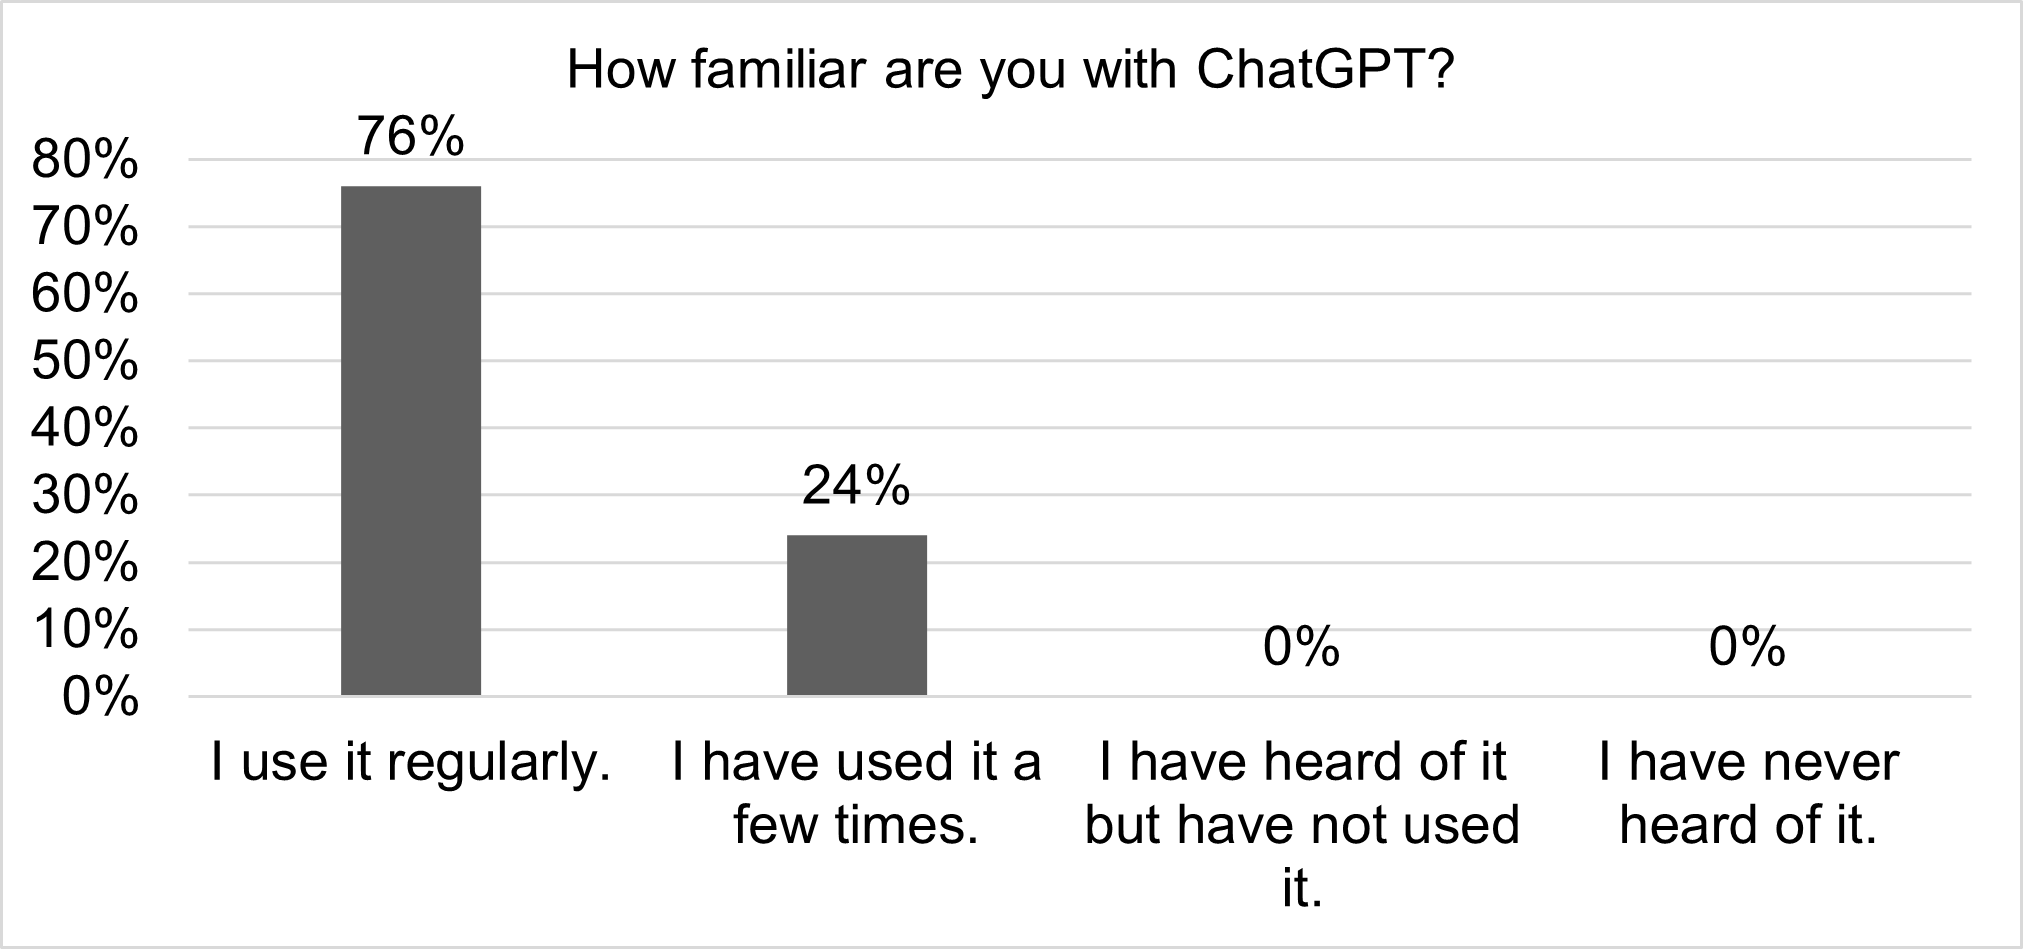
\includegraphics[width=\linewidth]{Imagens/FIGURA1.png}
    \caption{Students’ familiarity with ChatGPT.}
    \label{fig-1}
    \source{Own elaboration.}
    \end{minipage}
\end{figure}

As presented in Figure \ref{fig-1}, the results of the survey showed that a majority of the respondents (76\%) regularly used ChatGPT in their learning activities. A few of them (24\%) reported that they used it a few times, suggesting they were moderately aware of the platform. Interestingly, none of the respondents selected the options ‘I have heard of it but have not used it’ or ‘I have never heard of it’. These results seem to suggest the widespread awareness and adoption of ChatGPT and its integration into students’ lives.

Figure \ref{fig-2} presents the regularity of ChatGPT use for academic purposes. The participants’ responses to the frequency question suggest that ChatGPT was integrated into academic routines, with a majority (90\%) reporting either daily or weekly use. One participant commented that he uses it ``daily, like every 2 hours". This higher adoption of ChatGPT for academic purposes shows the tool’s relevance and value in supporting undergraduate academic activities. However, the remaining 10\% of respondents’ monthly use of the tool may reflect either situational or task-specific reliance on the tool.

%--- CÓDIGO DA FIGURA 2 ---%
\begin{figure}[h!]
    \centering
    \begin{minipage}{0.80\linewidth}
    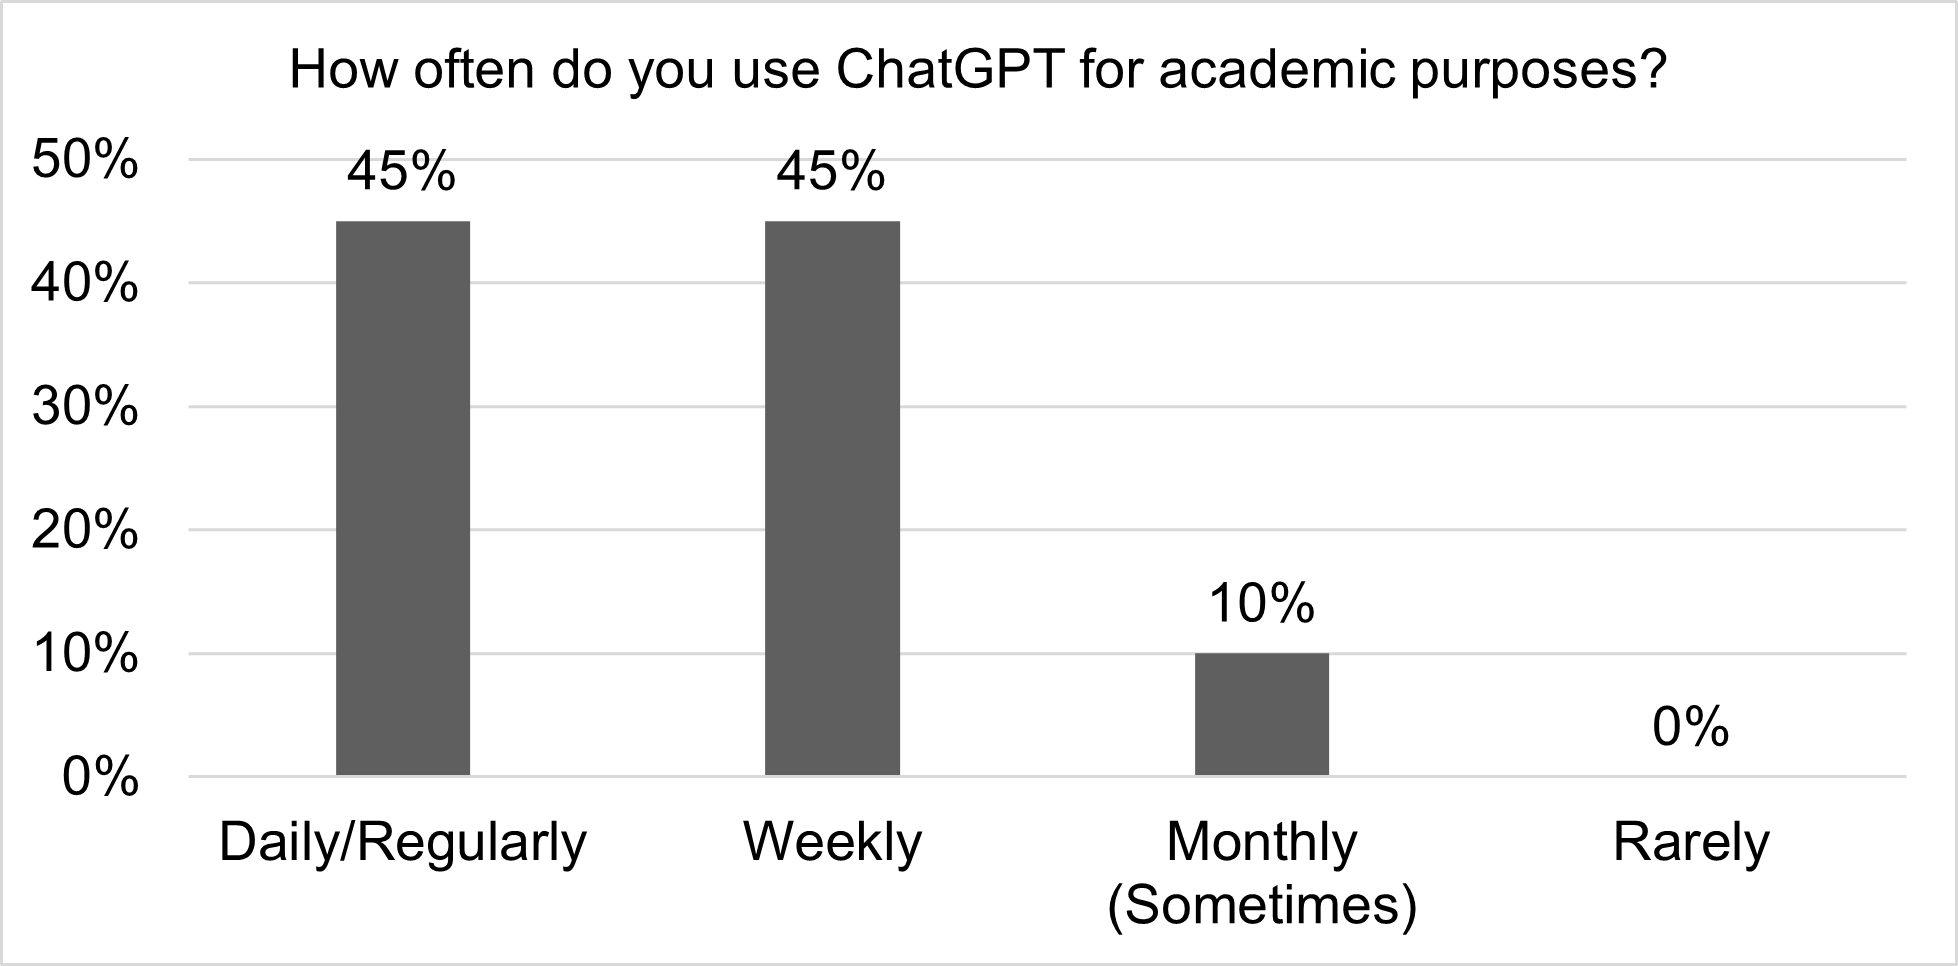
\includegraphics[width=\linewidth]{Imagens/FIGURA2.png}
    \caption{Frequency of ChatGPT use for academic purposes.}
    \label{fig-2}
    \source{Own elaboration.}
    \end{minipage}
\end{figure}



\subsection{Academic tasks and writing purposes}

%--- CÓDIGO DA FIGURA 3 ---%
\begin{figure}[h!]
    \centering
    \begin{minipage}{0.80\linewidth}
    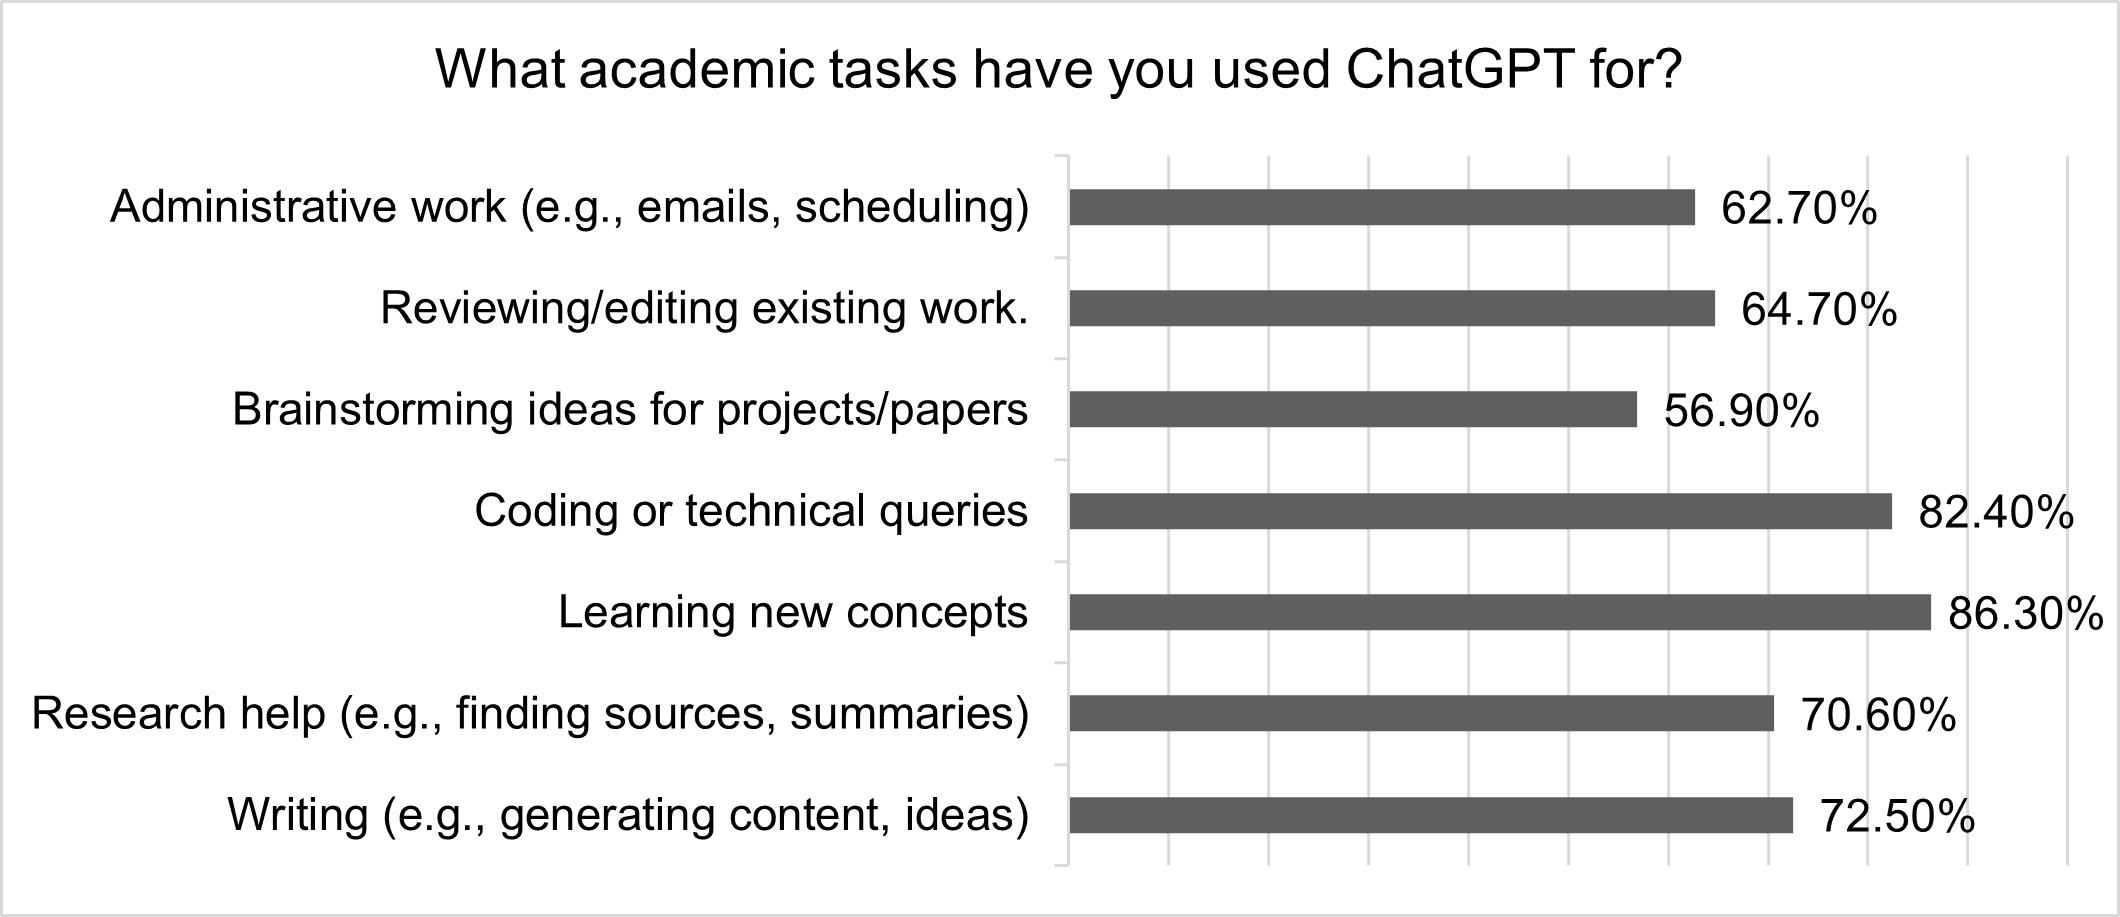
\includegraphics[width=\linewidth]{Imagens/FIGURA3.png}
    \caption{Academic applications of ChatGPT.}
    \label{fig-3}
    \source{Own elaboration.}
    \end{minipage}
\end{figure}

As presented in Figure \ref{fig-3}, the respondents reported that they used ChatGPT mostly for ‘learning new concepts’ (86\%) and ‘coding or technical queries’ (82\%), indicating the tool’s application in technical learning. However, one participant noted that “there are better AI tools than ChatGPT for technical work”. Other frequent tasks, such as ‘generating content and ideas’ (73\%) and ‘finding sources and summaries’ (71\%), demonstrate ChatGPT’s role in writing and research. The use of ChatGPT for tasks such as ‘reviewing/editing existing work’ (65\%) and ‘administrative work’ (63\%) suggests the tool’s capacity to support tasks related to review, revision and academic administration. Interestingly, just 57\% of the respondents reported that they used ChatGPT to ‘brainstorm ideas for projects/papers’, indicating students’ preference for employing ChatGPT for more structured tasks rather than open-ended ideation.

\newpage
From Figure \ref{fig-4}, it can be noted that a majority (80\%) of the respondents used ChatGPT both to generate new texts and review already written ones. The majority’s adoption of the tool for both purposes suggests a balanced application of ChatGPT. A small proportion of them (12\%) reported that they utilised ChatGPT mostly for reviewing tasks such as proofreading, editing, and improving the clarity and coherence of existing texts. The use of ChatGPT only for review and revision seems to stem from a ‘user-led’ interaction with the AI tool as it responds to and improves on the user’s prewritten texts. A smaller group of the participants (8\%) employed ChatGPT primarily for generating new texts. These students appear to be ‘AI-led’, where the user depends on ChatGPT to initiate and guide content creation. One concerned student noted that “people are losing their individuality by turning to ChatGPT before thinking of ideas themselves”. The over-reliance on ChatGPT for idea generation may lead to superficial learning habits and affect an individual’s intellectual autonomy.

%--- CÓDIGO DA FIGURA 4 ---%
\begin{figure}[h!]
    \centering
    \begin{minipage}{0.80\linewidth}
    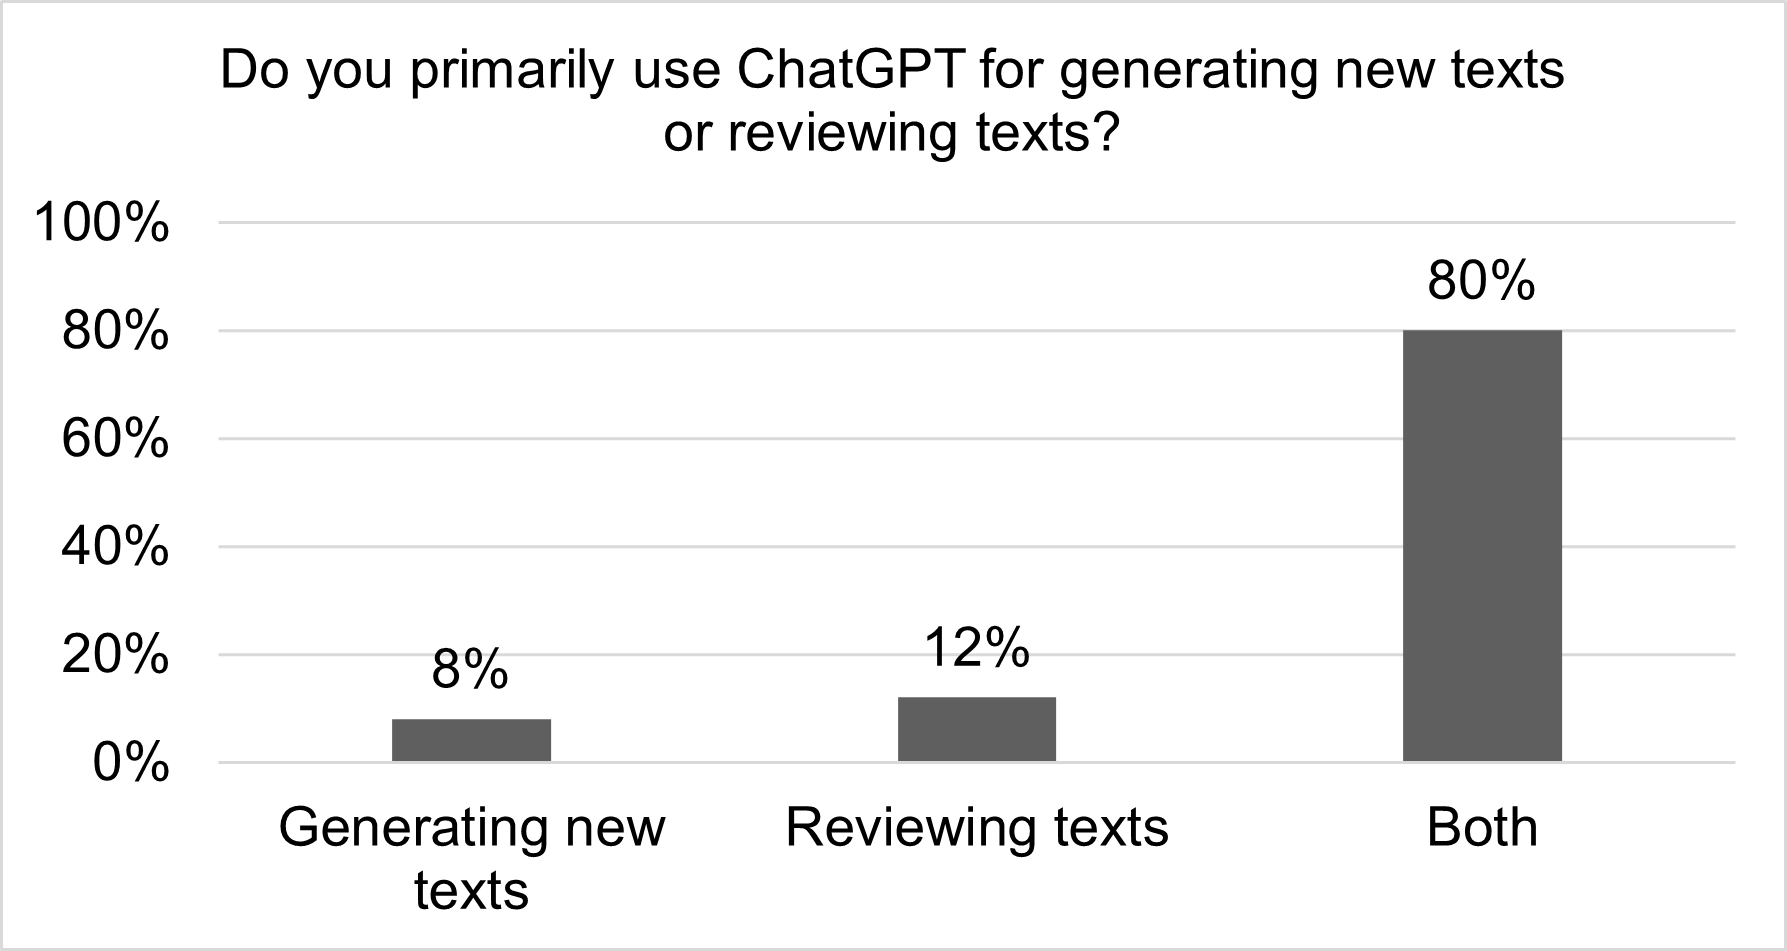
\includegraphics[width=\linewidth]{Imagens/FIGURA4.png}
    \caption{Writing purposes of using ChatGPT.}
    \label{fig-4}
    \source{Own elaboration.}
    \end{minipage}
\end{figure}


\subsection{Perceptions of ChatGPT’s usefulness, trustworthiness, and impact on academic writing}

The participants’ varying levels of perceived usefulness of ChatGPT for academic writing are presented in Figure \ref{fig-5}. More than half of the respondents (57\%) indicated a largely favourable perception of ChatGPT’s utility for academic writing, with 14\% rating it ‘extremely useful’ and 43\% finding it ‘very useful’. However, 43\% of the participants expressed a tempered view on its utility, with 41\% considering it ‘moderately useful’ and 2\% rating it ‘slightly useful’. One student remarked that it is ``[a] very useful tool though some improvements could be made to make it even more useful". None of them selected ‘not useful at all’, suggesting that they all found the tool valuable for academic writing tasks. However, the varying levels of perceived usefulness suggest that ChatGPT’s effectiveness may depend on an individual’s familiarity with it and the nature of the writing tasks being performed, as reinforced by a comment from a respondent: ``It is very useful if you know how to use it; prompt engineering is important to learn if you want to use it regularly and with good precision".

%--- CÓDIGO DA FIGURA 5 ---%
\begin{figure}[h!]
    \centering
    \begin{minipage}{0.80\linewidth}
    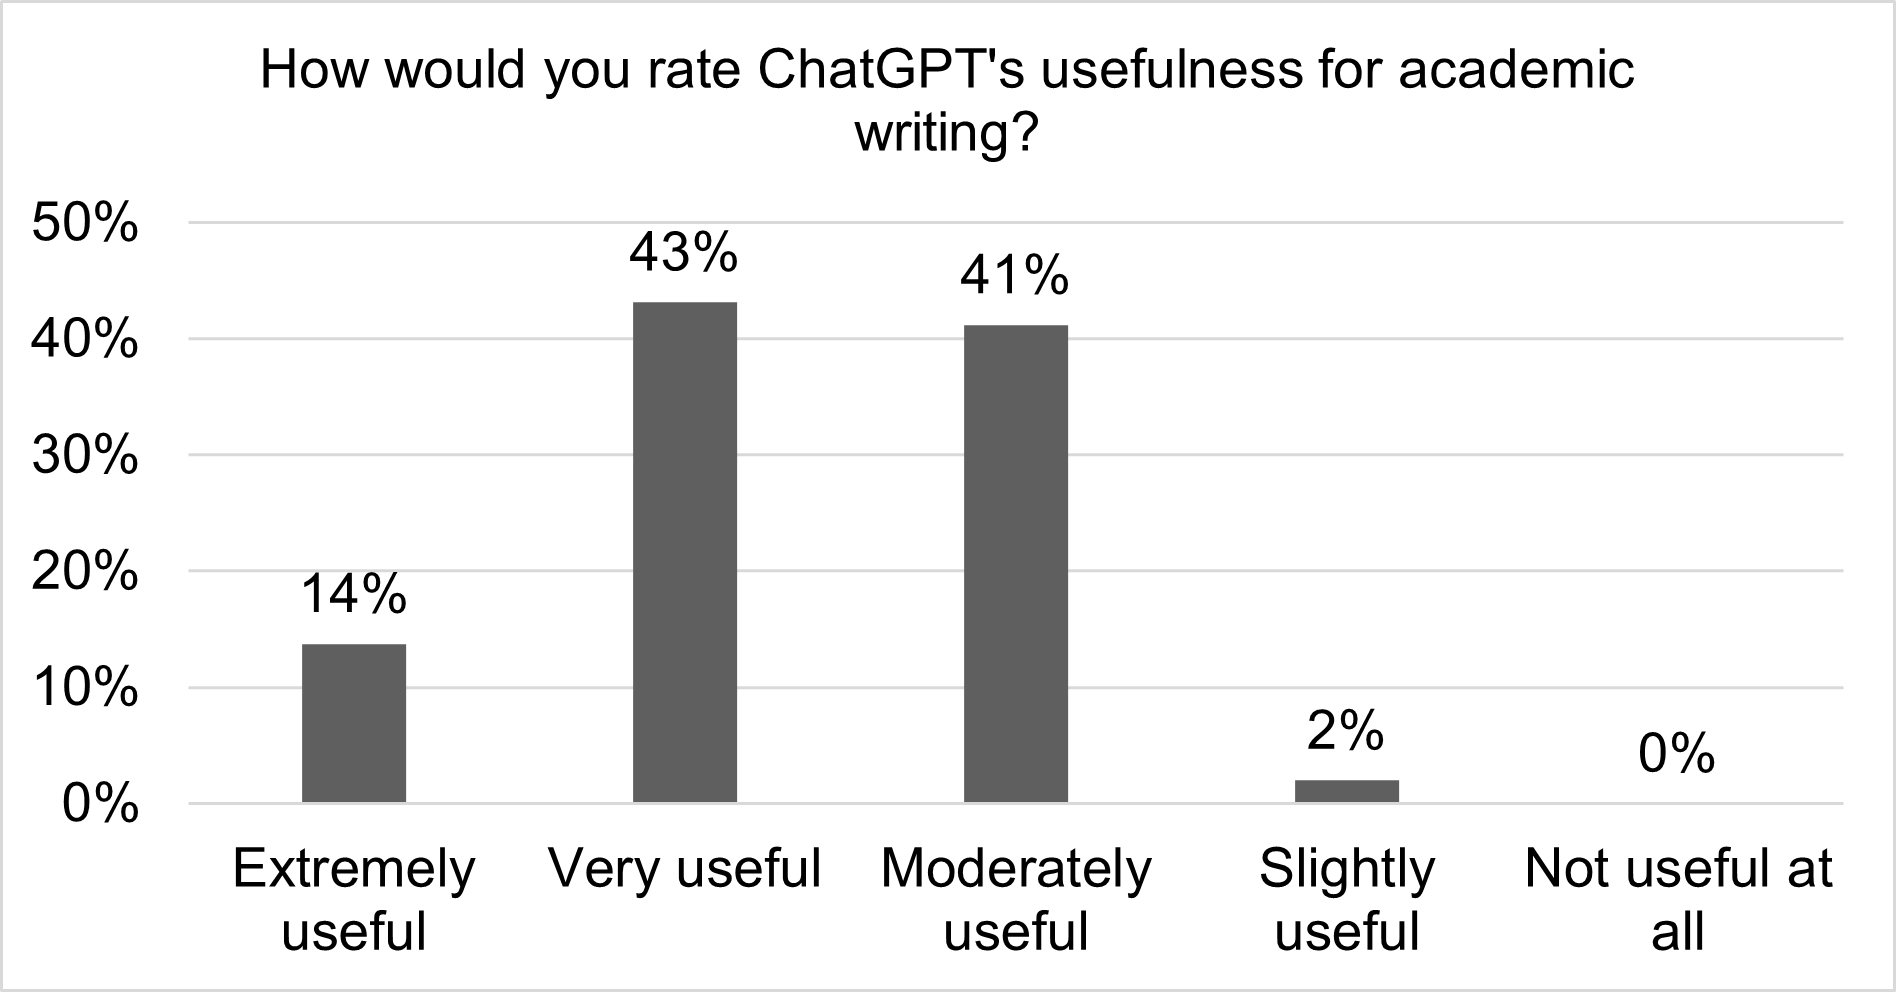
\includegraphics[width=\linewidth]{Imagens/FIGURA5.png}
    \caption{Students’ perceptions of ChatGPT’s usefulness.}
    \label{fig-5}
    \source{Own elaboration.}
    \end{minipage}
\end{figure}

The participants appeared to maintain a cautious optimism regarding the trustworthiness of information provided by ChatGPT for academic writing tasks. As shown in Figure \ref{fig-6}, though none of them rated ChatGPT’s information as ‘completely trustworthy’, more than half of the respondents (55\%) found the information to be ‘somewhat trustworthy’, indicating a cautious reliance on ChatGPT. A notable portion of the participants (43\%) rated it ‘mostly trustworthy’, and one participant noted that ``it is growing with the enormous rise in computational capabilities … so I think we should trust technology". However, 2\% of the respondents viewed the information as ‘not trustworthy’, probably because, as one student noted, the ``factual information is generally wrong". While most respondents acknowledge some level of trust, there is substantial caution in considering it entirely dependable.

%--- CÓDIGO DA FIGURA 6 ---%
\begin{figure}[h!]
    \centering
    \begin{minipage}{0.80\linewidth}
    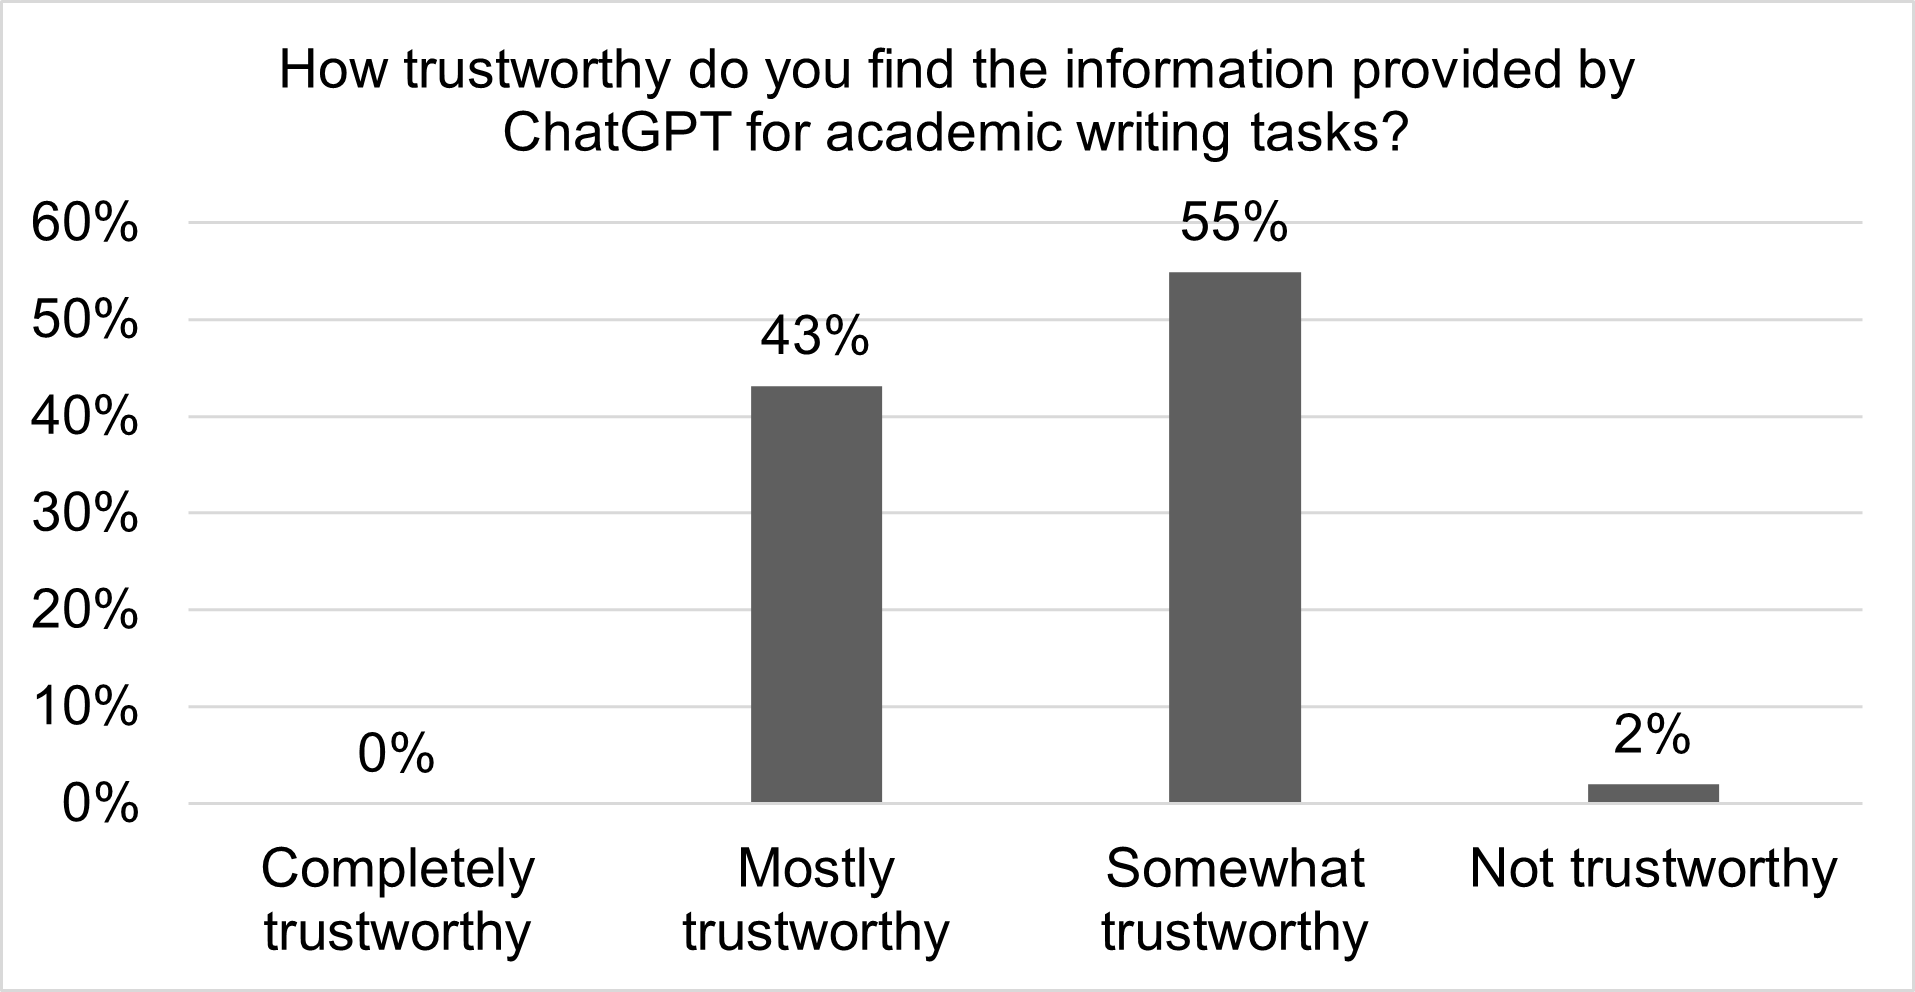
\includegraphics[width=\linewidth]{Imagens/FIGURA6.png}
    \caption{Students’ views on ChatGPT’s trustworthiness.}
    \label{fig-6}
    \source{Own elaboration.}
    \end{minipage}
\end{figure}

Figure \ref{fig-7} shows the participants’ perceptions of ChatGPT’s impact on academic writing. A little over 80\% of the participants perceived ChatGPT as a positive influence on their academic writing, with 19.6\% ‘strongly agreeing’ and 60.8\% ‘agreeing’ with the statement on ChatGPT’s contribution to their academic writing. Since ChatGPT synthesises information from various sources, it can save students a lot of time. One of the respondents commented that ``ChatGPT makes a lot of things easy and fast. We can directly access what we want to know rather than searching across multiple websites on Google". Further, 19.6\% of respondents were neutral, showing neither strong support nor disapproval, and no respondents ‘disagreed’ or ‘strongly disagreed’ with the statement on its enhancement of academic writing. Overall, despite the presence of neutral responses by a fifth of participants, the data appears to highlight a general consensus on ChatGPT’s moderately positive impact on academic writing productivity.

%--- CÓDIGO DA FIGURA 7 ---%
\begin{figure}[h!]
    \centering
    \begin{minipage}{0.80\linewidth}
    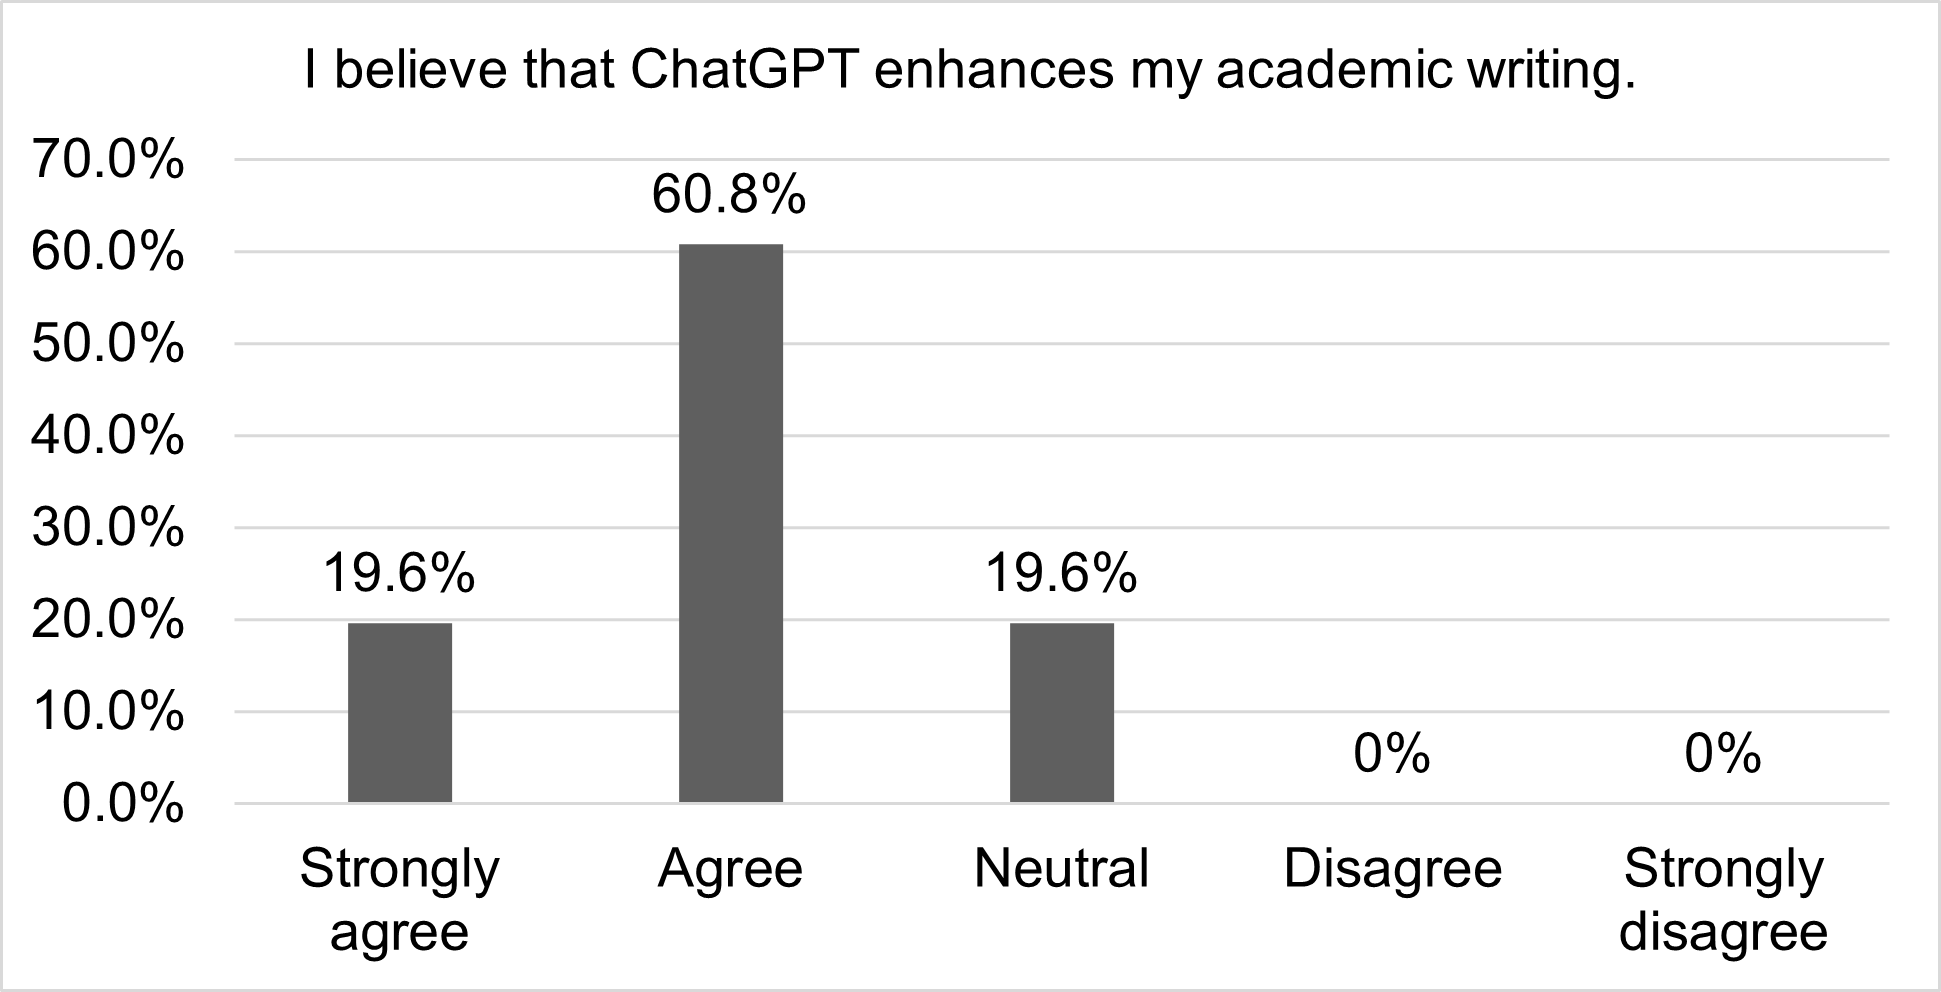
\includegraphics[width=\linewidth]{Imagens/FIGURA7.png}
    \caption{Students’ beliefs about ChatGPT’s impact on academic writing.}
    \label{fig-7}
    \source{Own elaboration.}
    \end{minipage}
\end{figure}

\subsection{Confidence and willingness}

%--- CÓDIGO DA FIGURA 8 ---%
\begin{figure}[h!]
    \centering
    \begin{minipage}{0.80\linewidth}
    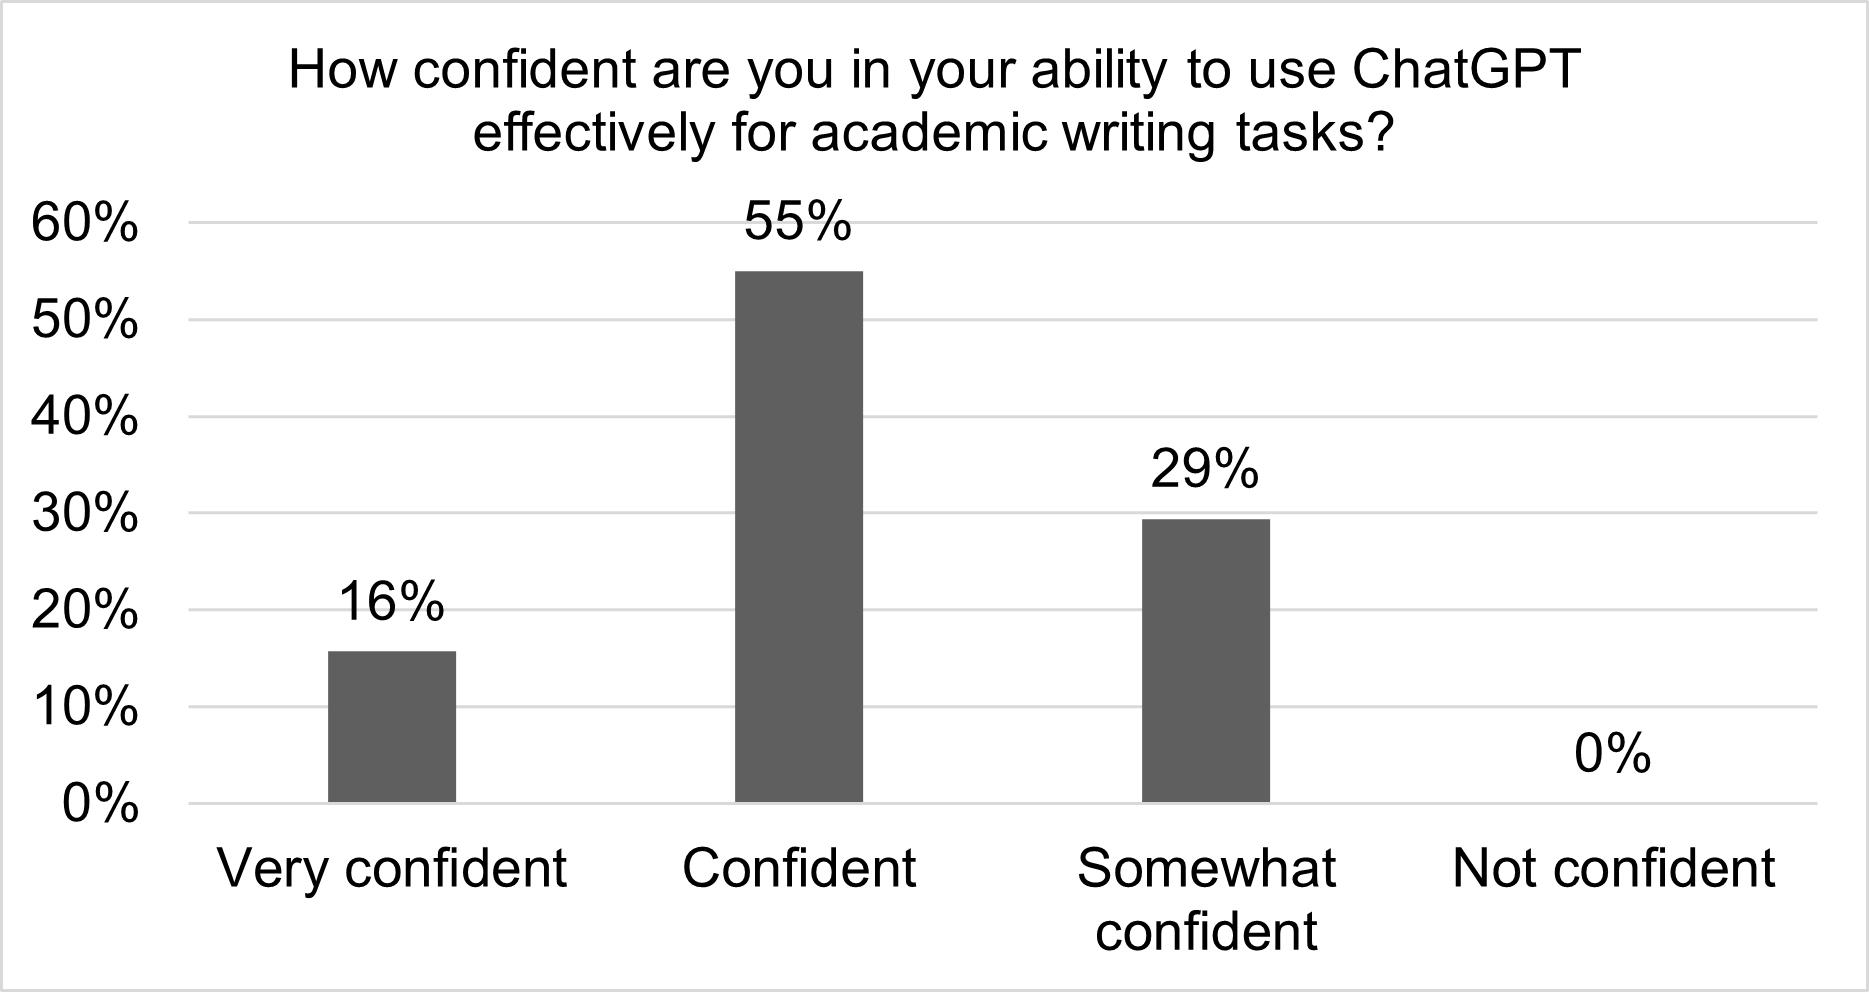
\includegraphics[width=\linewidth]{Imagens/FIGURA8.png}
    \caption{Students’ confidence in using ChatGPT for academic writing tasks.}
    \label{fig-8}
    \source{Own elaboration.}
    \end{minipage}
\end{figure}

Regarding the confidence levels in using ChatGPT effectively for academic writing, 55\% of the respondents said they were ‘confident’ and 16\% reported being ‘very confident’ (Figure \ref{fig-8}). These confidence levels among most participants show that they were adequately equipped to use ChatGPT for their academic writing. However, 29\% of the respondents described themselves as ‘somewhat confident’. This uncertainty about their confidence suggests that they may have occasional doubts and challenges in using ChatGPT for academic writing tasks.

%--- CÓDIGO DA FIGURA 9 ---%
\begin{figure}[h!]
    \centering
    \begin{minipage}{0.80\linewidth}
    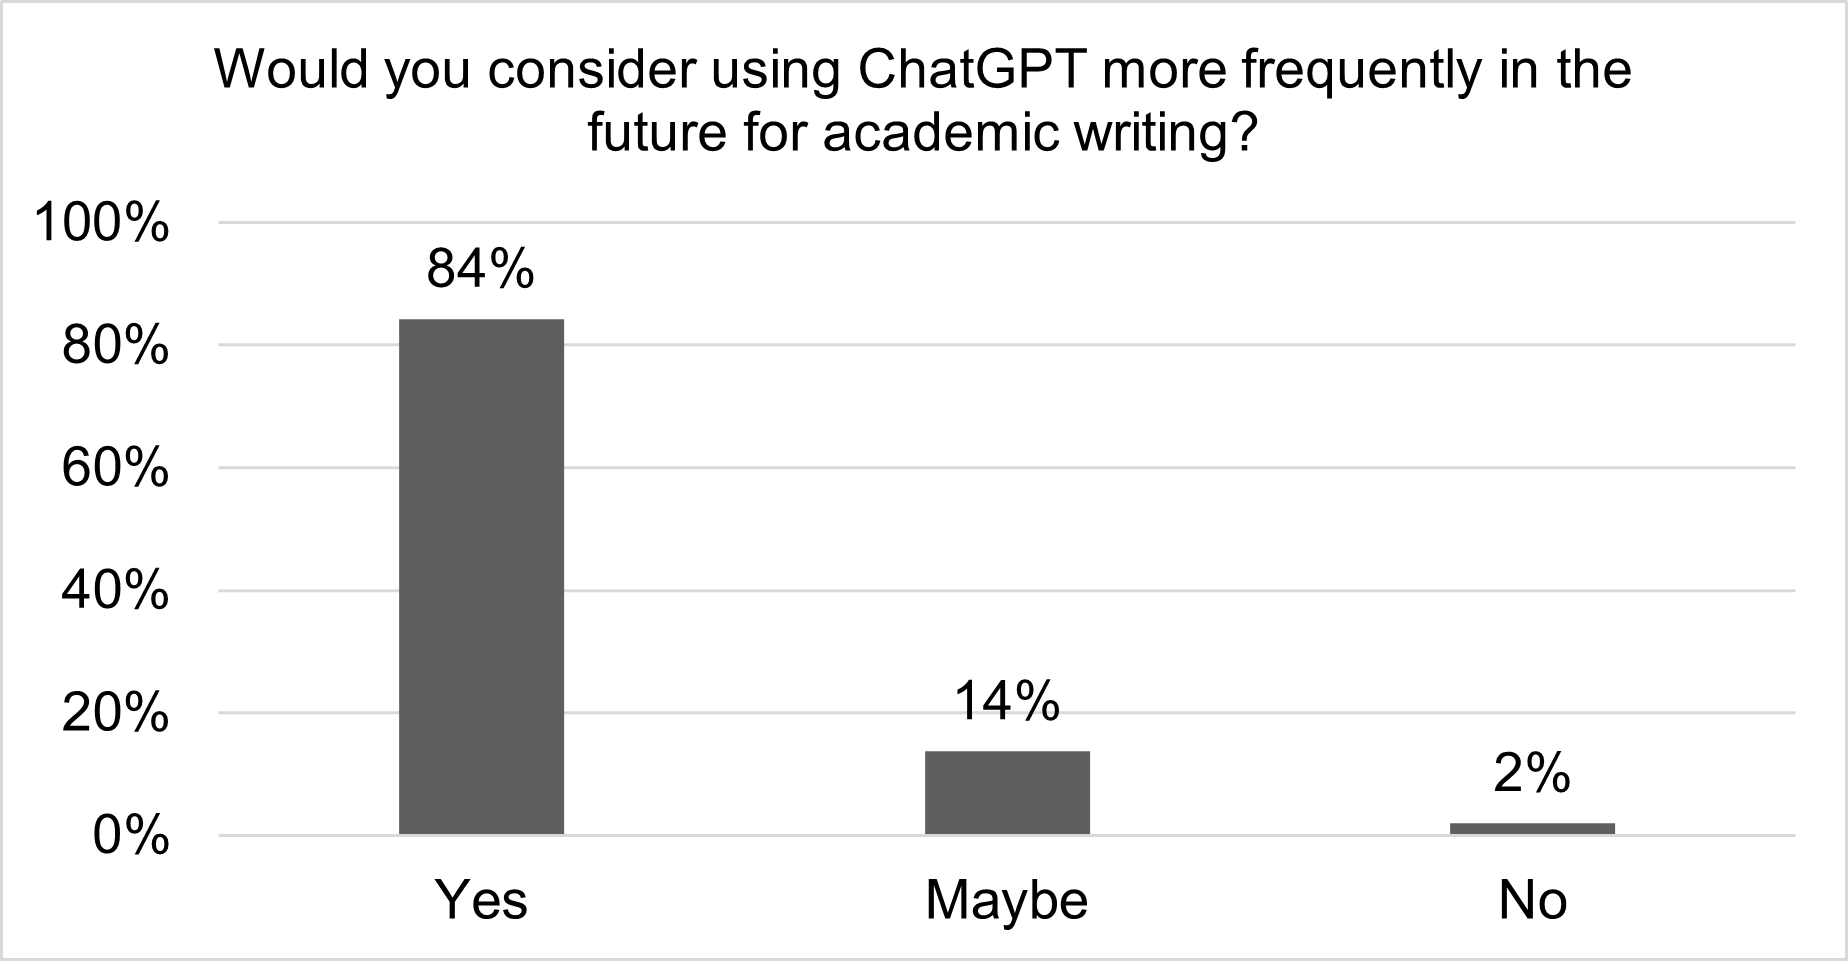
\includegraphics[width=\linewidth]{Imagens/FIGURA9.png}
    \caption{Students’ willingness to increase ChatGPT use.}
    \label{fig-9}
    \source{Own elaboration.}
    \end{minipage}
\end{figure}

As shown in Figure \ref{fig-9}, a majority of the respondents (84\%) expressed willingness to use ChatGPT more frequently for academic writing in the future. The majority’s willingness indicates ChatGPT’s capabilities to improve students’ academic writing performance. However, 14\% of the participants reported uncertainty (Maybe) and 2\% unwillingness (No) to increase the use of ChatGPT, probably due to its limitations and unreliability. One student, particularly, cautioned not to ``completely rely on AI" because it can make mistakes.

\subsection{Findings from cross-analysis}\label{sec-4_5}

Cross-analysis of the data reveals that among students who identified as ‘Very confident’ (n=8), 62.5\% rated ChatGPT as ‘Extremely useful’. Among students who reported being ‘Confident’ (n=28), 53.6\% rated ChatGPT as ‘Very useful’ and 35.7\% as ‘Moderately useful’. Similarly, 53.3\% of ‘Somewhat confident’ users (n=15) rated ChatGPT as ‘Moderately useful’ and 46.7\% as ‘Very useful’. While the subgroup sizes are small, the data seem to suggest that the perceived usefulness of ChatGPT tends to increase with students’ confidence levels, indicating a probable relationship between the two variables. Moreover, most students who rated ChatGPT as ‘Mostly trustworthy’ (n=22) showed strong intent to use it more frequently, with 95.5\% affirming this and only 4.5\% selecting ‘Maybe’. By comparison, of those who found it ‘Somewhat trustworthy’ (n=28), 75.0\% expressed a strong intention to use it, while 21.4\% selected ‘Maybe’. These numbers seem to suggest a possible link between perceived trustworthiness and students’ intention to use ChatGPT in the future.

\section{Discussion}
The findings presented in the previous section have outlined undergraduate ESL students’ use and perceptions of ChatGPT for academic writing purposes. This section interprets and contextualises those findings in light of relevant literature. For clarity and ease of reading, the discussion is organised into thematic subsections, mirroring the structure used in the findings section.

\subsection{Familiarity and frequency}
The survey showed that a majority of the respondents were familiar with ChatGPT, which can be attributed to its accessibility and user-friendliness. However, such high adoption rates can increase overdependence, which could, as noted by \textcite{mogavi2024}, undermine students’ independent learning efforts and imply the need to teach students how to use AI tools judiciously. The current research also indicated that a majority of respondents engaged with ChatGPT regularly for their academic tasks, revealing its widespread presence and adoption in ESL contexts. These findings comply with the results of previous research \cite{crcek2023, klimova2024, punar2024}, which emphasise the growing role of ChatGPT in educational settings, but contradict \textcite{mahapatra2024} pre-experiment observation that his undergraduate participants did not use ChatGPT to improve their writing skills.

\subsection{Academic tasks and writing purposes}
The participants’ responses indicate that ChatGPT was used for a variety of academic tasks, including learning new concepts, coding, generating texts, and reviewing their writing. These tasks have been reported in other studies as well (see \textcite{alkamel2024, crcek2023, higgs2024, klimova2024, punar2024}). These findings are in line with the observations of previous researchers \cite{robillos2024, teng2024a}, who noted ChatGPT’s potential as a multipurpose academic tool. However, concerns about diminishing originality due to its overuse for idea generation were found, and such heavy reliance on AI for ideation, as cautioned by \textcite{chia2024}, could stifle intellectual autonomy and novelty.

The study reveals that a majority of respondents appeared to adopt a balanced approach to leveraging ChatGPT’s capabilities for both generating new texts and revising existing ones, while some used it exclusively either for the former or the latter. These findings regarding the academic writing purposes of using ChatGPT can be understood from three metaphors: integrator, dependent and evaluator. Integrators interact dynamically with ChatGPT by balancing their own input with AI assistance to produce texts that are moderately human-generated and characterised by a blend of creation and evaluation. This dual use demonstrates the adaptability of ChatGPT at different stages of the writing process, a finding consistent with the discoveries of \textcite{mahapatra2024} and \textcite{xiao2023}. Dependents engage minimally with ChatGPT for their writing improvement, act as passive prompters with little critical input, and rely heavily on the tool to generate content, resulting in largely AI-generated texts. This dependency behaviour, as reported and discussed by previous researchers \cite{alkamel2024, klimova2024, mogavi2024, teng2024b, yuan2024}, can diminish critical thinking and social skills. Evaluators engage with ChatGPT as architects of their writing and use the tool primarily to evaluate and refine their writing, demonstrating high levels of critical thinking \cite{koltovskaia2024, lee2024}. The study’s finding about the presence of ChatGPT dependents among undergraduates implies the need to train students to progress from their dependency on it to the evaluator level.

\subsection{Perceptions of ChatGPT’s usefulness, trustworthiness, and impact on academic writing}
Findings show that students appeared to have a positive perception of ChatGPT’s usefulness for academic writing. Previous researchers \cite{abusaaleek2024, alkamel2024, bekturova2025, duong2025, klimova2024} identified ChatGPT’s role in improving efficiency and enhancing academic productivity. However, some students thought that the tool’s features could be advanced to make it even more useful. Despite its perceived usefulness, the study found cautious optimism regarding ChatGPT’s trustworthiness. While a majority of the participants found its information moderately trustworthy, none of them completely trusted its responses. This scepticism might be the result of broader concerns about the accuracy of AI-generated responses \cite{bekturova2025, higgs2024, teng2024a}. \textcite{meniado2024} recommended a critical evaluation of AI-generated responses and adequate training in prompt engineering to maximise the tool’s utility. The findings also show that four in five believed that ChatGPT enhanced their academic writing. This finding is in agreement with previous research \cite{crcek2023, mahapatra2024} that showed ChatGPT’s role in improving organisation, accuracy, and grammar, fostering collaboration, and supporting learner autonomy. However, one-fifth of neutral respondents suggest that the degree of writing enhancement may depend on students’ digital literacy and individual choices.

\subsection{Confidence and willingness}
The study’s findings show that most students were reasonably confident in employing ChatGPT for academic writing purposes. However, nearly one in three expressed relatively lower levels of confidence, and this uncertainty suggests occasional challenges in appropriately prompting the tool. These prompting challenges can result from their limited experience with the tool’s features and a lack of training in prompt engineering and AI literacy \cite{mahapatra2024}. Therefore, there is a need for training to help them improve their skills and leverage ChatGPT for academic tasks more confidently. Several researchers \cite{meniado2024, punar2024, teng2024a} have called for training programs on leveraging AI tools such as ChatGPT to improve undergraduate students’ writing skills.

The study’s participants appeared to demonstrate a moderate willingness to increase their use of ChatGPT for academic writing purposes in the future, probably due to its ability to augment their writing experiences and academic achievement. However, a small proportion of participants expressed hesitation and concerns about the reliability of its responses and the possible dangers of overdependence, both risks that were emphasised by \textcite{higgs2024} and \textcite{mogavi2024}. The impact of these risks can be lowered when teachers provide designed support to help students use ChatGPT effectively and ethically \cite{teng2024a}. The training can focus on how students can critically engage with ChatGPT as a review and refinement tool rather than use it to generate texts.

\subsection{Study’s contribution}
The study’s findings add to the growing body of literature on ChatGPT by exploring its academic application among Indian undergraduate ESL students -- a demographic often underrepresented in research on AI-assisted writing tools \cite{mahapatra2024}. While most of the existing studies investigated ChatGPT’s role in general ESL writing contexts \cite{al-alami2024, allen2024, teng2024b}, the current study surveyed how ESL students perceive and utilise the tool specifically for academic writing purposes. By investigating students’ perceptions of ChatGPT’s usefulness and trustworthiness, the study addresses the gaps indicated in previous research \cite{mahapatra2024, teng2024a} in understanding how ESL undergraduates interact with AI tools to support their academic performance. Additionally, the study corroborates the findings of previous research \cite{abusaaleek2024, bekturova2025, mogavi2024, teng2024b, yuan2024} by revealing the duality of ChatGPT’s role as both a support tool and a potential source of dependency. While earlier literature \cite{higgs2024, mogavi2024, shoufan2023, szabo2024, yuan2024} cautioned about the risks of developing shallow learning habits due to overreliance, this study contextualises these concerns within an ESL academic writing context, discovering the situated benefits and challenges of using ChatGPT for academic writing tasks.

The current study contributes in distinct ways to the increasing volume of scholarship on ESL students’ use and perceptions of ChatGPT. While \textcite{abusaaleek2024} focused on postgraduate learners, this research examines undergraduate ESL students -- a group with different levels of academic maturity and learning needs. Similarly, while \textcite{alkamel2024} examined the perceptions of Yemeni EFL learners, the current research concentrates on Indian undergraduate STEM students, offering an understanding of a geographically and academically distinct population that remains underrepresented in AI-assisted academic writing research. Furthermore, while \textcite{mahapatra2024} explored Indian students' perceptions of ChatGPT primarily as a feedback tool, this study adopts a broader lens that includes perceptions as well as usage frequency, familiarity, trustworthiness, confidence, and willingness to adopt ChatGPT in academic writing. These additional dimensions allow for a more thorough understanding of how undergraduate ESL learners engage with AI tools in academic contexts.

\subsection{Limitations and recommendations for future research}
Though the study contributes to the literature on ChatGPT for academic writing, the following limitations may be noted. First, a self-reporting survey was employed as a data collection tool. When participants self-report, they might either overreport or underreport their familiarity or confidence in using ChatGPT. Second, the study followed a purposive sampling technique and selected an intact class of an academic writing course to collect authentic and valid data. While the class had students from diverse STEM disciplines, educational backgrounds, and English proficiency levels, participants from other types of educational institutes may have different experiences with ChatGPT. Future research may explore perceptions of students from other disciplines, such as humanities, social sciences and management, and other types of educational institutions, to capture a larger variety of perceptions toward ChatGPT. Third, the study used predominantly a quantitative survey. While it was useful for identifying the generalised trends and perceptions, it might not have captured the experiences and attitudes of individual students comprehensively. Though one open-ended question generated qualitative data on individual perspectives, future research could include more qualitative questions, as well as in-depth interviews or focus group discussions, to enrich the findings. Last, given the unequal and small gender subgroups in the sample, the study could not perform inferential statistical comparisons based on gender. Future research with a larger sample may examine potential gender-based differences in students’ use and perceptions of ChatGPT for academic writing.

\subsection{Implications}
Despite the study’s limitations, its findings have implications for educators, policymakers, and ChatGPT developers. For educators, the findings about ChatGPT’s utility for academic tasks imply the need to integrate AI literacy modules into academic writing instruction to teach students when, how, and why to use ChatGPT effectively. However, students’ genuine concerns about developing shallow learning habits due to overreliance on such AI-driven writing tools suggest that students need to be adequately trained to use such tools to boost their academic productivity while also maintaining independence in their learning. The study’s findings also imply that administrators of educational institutions, rather than banning AI writing tools, need to develop ethical protocols for ChatGPT’s use in academic contexts to ensure its prudent use for academic writing. Furthermore, the findings regarding students’ authentic doubts about ChatGPT’s reliability and trustworthiness imply that its developers should improve its contextual precision and response correctness to make it more reliable and accurate.

Above all, the findings have specific implications for AI literacy training interventions and programmes. The components of a training course for students on leveraging AI tools for academic writing could include ``awareness", ``prompt engineering", ``criticality" and ``ethicality". First, students could be made aware of the strengths and weaknesses of AI tools such as ChatGPT to help them decide when to use and avoid them for academic writing. Second, because prompts can shape the kind of output these AI tools produce, students could be trained in designing and modifying prompts based on their needs and goals of writing. Third, as participants were concerned about the reliability and trustworthiness of the AI-generated responses, students need to be taught to critically review the outputs of AI tools, verify their responses with more reliable sources, and evaluate their correctness, relevance, and appropriateness. Last, to uphold academic integrity, learners could be made aware of ethical procedures such as avoiding misuse of AI tools, refraining from using them only for generating texts like AI-dependents, referencing appropriately and complying with institutional policies. However, it may be noted that these four components are not exhaustive, and future research could add more components to develop a comprehensive AI literacy training programme for academic writing.

\section{Conclusion}
This study surveyed undergraduate ESL students’ use and perceptions of ChatGPT for academic writing purposes, particularly their familiarity with ChatGPT, its applications, and their observations about its effectiveness, trustworthiness and utility. The findings indicate that most of the participants regularly used ChatGPT for academic purposes, including generating and reviewing texts. They expressed watchful confidence regarding the trustworthiness of responses provided by ChatGPT for academic writing tasks and acknowledged its utility in academic writing. While their confidence levels in using ChatGPT showed modest variation, most of them were willing to use it more frequently for academic writing in the future. The findings reflect students’ contrasting perspectives towards ChatGPT as a writing tool, encompassing both its strengths and limitations. Thus, the study adds to an ever-growing body of literature on AI-driven writing assistance tools by discovering ESL students’ patterns of use and perceptions of ChatGPT for academic writing purposes.


\printbibliography\label{sec-bib}
% if the text is not in Portuguese, it might be necessary to use the code below instead to print the correct ABNT abbreviations [s.n.], [s.l.]
%\begin{portuguese}
%\printbibliography[title={Bibliography}]
%\end{portuguese}





\end{document}

